%%=====================================================================
%%  AIAgNav --- IEEE ICRA 2027 submission
%%
%%  SINGLE-FILE OVERLEAF SOURCE.  Upload this one .tex and nothing else.
%%
%%  How to use on Overleaf:
%%    1. overleaf.com  ->  New Project  ->  Upload Project  (or Blank
%%       Project, then drag this file in).
%%    2. Menu -> Compiler: pdfLaTeX.  Main document: this file.
%%    3. Recompile.  It builds clean with zero errors.
%%
%%  Deliberately self-contained:
%%    * No \bibliography / .bib file. References are a thebibliography
%%      environment at the end, so there is no BibTeX pass to go wrong.
%%    * No \includegraphics of external files. Both diagrams are TikZ
%%      drawn inline, so nothing can be "missing".
%%    * Pure ASCII. No inputenc/UTF-8 surprises on any compiler.
%%
%%  Two-column layout, IEEE fonts and spacing come from the class option
%%  [conference] on IEEEtran below. Do not switch to article.
%%
%%  HARD LIMIT: 8 pages including references.
%%=====================================================================

\documentclass[conference]{IEEEtran}
\IEEEoverridecommandlockouts

\usepackage{amsmath,amssymb}
\usepackage{graphicx}
\usepackage{booktabs}
\usepackage{url}
\usepackage{cite}
\usepackage{tikz}
\usetikzlibrary{arrows.meta,positioning,calc}

%% Unresolved facts render visibly in the PDF so they cannot slip through.
\newcommand{\TODO}[1]{\textbf{[TODO: #1]}}

\begin{document}

\title{AIAgNav: A Semantic Segmentation-Based Autonomous\\
       Navigation System for Cornfields}

\author{\IEEEauthorblockN{Wei-Wei Chien, Author Two, and David J. Cappelleri}
\IEEEauthorblockA{School of Mechanical Engineering, Purdue University,
West Lafayette, IN 47907 USA\\
\texttt{\{chien21, cappelleri\}@purdue.edu}}%
\thanks{This work was supported by \TODO{funding source and grant number}.}}

\maketitle

%%=====================================================================
%% ABSTRACT
%%=====================================================================
\begin{abstract}
Under-canopy navigation in cornfields must be closed on onboard perception:
the corridor between rows is under a metre wide and GNSS degrades exactly where
the canopy is densest. Existing under-canopy systems solve this with 3D LiDAR,
which measures geometry and cannot separate a rigid stalk from a leaf hanging
into the corridor. This paper presents AIAgNav, a navigation system that drives
a ground robot in-row, under-canopy, and across multiple rows from a single
monocular RGB camera. A DINOv3 backbone with a mask transformer head segments
each frame into sky, traversable ground and obstacle; closed-form geometry
reduces the mask to a lateral error and a heading proxy; and a receding-horizon
model predictive controller in normalized image coordinates issues the steering
command, with no filter, no camera calibration and no state estimator in
between. A mission layer detects the end of a row from the same mask, turns onto
the headland, re-enters the next row, and reverses out of blocked rows. The
system is evaluated in simulation and in a real cornfield,
\TODO{headline result: distance covered, rows completed, MDBI}.
\end{abstract}

\begin{IEEEkeywords}
Robotics and automation in agriculture and forestry, agricultural automation,
semantic segmentation, visual navigation, model predictive control.
\end{IEEEkeywords}

%%=====================================================================
%% I. INTRODUCTION
%%=====================================================================
\section{Introduction}
Precision agriculture depends on measurements taken close to the plant, and the
measurements that matter most for breeding and nutrient management---stalk
diameter, lower-leaf condition, soil surface state---are the ones the canopy
hides~\cite{ref07,ref08}. Aerial platforms and high-clearance tractors observe a
field from above and lose access to the plant interior as the season
advances~\cite{ref09}. An under-canopy ground robot is the most direct route to
per-plant measurement in row crops: a robot small enough to drive between two
corn rows reaches the stalk, the lower leaves and the soil surface directly, and
can carry a sampling arm to the plant rather than the plant to the
laboratory~\cite{kim2022pagbot,ref18}.

The environment such a robot must drive in is among the least forgiving
available to a mobile robot. The corridor between two rows of mature corn is
under a metre wide, bounded by plants rigid enough to damage a robot and
flexible enough to sweep across its sensors, and lit by a canopy that produces
order-of-magnitude illumination changes over a few metres of travel. Classical
map-and-plan navigation is a poor fit: hanging leaves and weeds that were absent
when a map was built register as obstacles, and the planner either detours
around growth the robot could simply drive through or fails
outright~\cite{ref12}. GNSS, which carries most agricultural autonomy above the
canopy~\cite{ref10,ref11}, degrades under it exactly where the corridor is
narrowest, because the plants that define the corridor also block and reflect
the signal. Navigation under the canopy therefore has to be closed on onboard
perception.

This work follows a line of under-canopy systems developed on the same platform.
P-AgBot~\cite{kim2022pagbot} centres the robot in a row by balancing left and
right distances from a 2D LiDAR and demonstrates in-row physical sampling.
P-AgSLAM~\cite{kim2024pagslam} builds an under-canopy state estimate from 3D
LiDAR features. P-AgNav~\cite{kim2025pagnav} extends that sensing into a
complete navigation system: it projects the 3D point cloud into a range view,
extracts the row corridor from that image, and sequences in-row driving,
end-of-row detection and headland turning into multi-row missions without GNSS
or pre-defined waypoints. The navigation problem in a cornfield is, in that
sense, not open. What this work questions is the sensor the solution is built
on.

A range sensor measures geometry, and the question a row-following controller
asks is not geometric. A return at 0.6\,m to the left of the robot is the same
measurement whether it came from a stalk, which must be avoided, or from a leaf
hanging into the corridor, which the robot drives through several times a
minute; no post-processing of the point cloud recovers a distinction that was
never measured. The consequence is that a geometric system must treat the
corridor conservatively, and that its notion of the row end is a matter of where
returns stop rather than of what the robot is looking at. A 3D LiDAR is also the
most expensive component on the robot by a wide margin, which matters for a
platform intended to be deployed in numbers across a research farm.

Camera-based under-canopy navigation addresses the semantic gap and has taken
two broad forms. The first regresses the navigation state directly from the
image. CropFollow~\cite{sivakumar2021cropfollow} predicts heading and lateral
distance from a monocular frame with a learned predictor and fuses the estimate
with inertial measurements in a filter; the approach is robust and has been
demonstrated over long distances, but it places the entire navigation state
inside a network whose failures are difficult to inspect and whose training set
must be large. The second extracts an explicit geometric structure from an
intermediate representation. Agronav~\cite{panda2023agronav} segments the
traversable region and fits a semantic line to it, an approach much closer to
the one taken here, but is developed for above-canopy field roads and inter-row
lanes rather than for the occluded, low-contrast interior of a mature corn row.
Classical crop-row detection from images~\cite{ref13} shares that limitation.
Neither line of work addresses the full multi-row mission---exit, headland turn,
re-entry, and recovery when the row is blocked---which is what separates a row
follower from a system that can cover a plot.

AIAgNav is a monocular, camera-only navigation system for that setting. A single
forward-facing RGB frame is segmented into sky, traversable ground and obstacle
by a DINOv3~\cite{simeoni2025dinov3} backbone with a mask transformer head,
chosen for label efficiency because the annotations must be produced by hand
from footage of the target field. The mask is reduced to a two-element
navigation state by closed-form geometry rather than by a learned regression
head, and that state is consumed directly by a receding-horizon model predictive
controller formulated in normalized image coordinates. A mission layer detects
the end of the row from the same mask, turns onto the headland, re-enters the
next row, and reverses out of rows that are blocked rather than finished. No
GNSS, no map, no waypoints, no camera calibration and no LiDAR are used at any
stage. Fig.~\ref{fig:pipeline} shows the resulting pipeline.

The contributions are:

\begin{itemize}
\item A complete in-row and multi-row cornfield navigation system driven by a
single low-cost monocular camera, with a second identical camera used only for
reverse and headland manoeuvres. The control problem is posed entirely in
normalized image coordinates, so no intrinsics, extrinsics or metric scale enter
the control law.
\item A navigation state read off a semantic segmentation mask by geometry
rather than regression, giving a lateral error and a heading proxy from a single
frame, at several depths, with no filter and no inertial input between
perception and control.
\item A mission layer for multi-row operation whose end-of-row evidence
accumulates in metres and seconds rather than in frame counts, so that one set
of thresholds transfers unchanged between robots whose inference rates differ by
an order of magnitude, together with a rear-view-steered headland leg and a
blocked-row reverse recovery.
\end{itemize}

GNSS is used nowhere in the system described here. An RTK receiver is planned
for the above-canopy transit from the field edge to the row entrance, which is
the one regime in which it is reliable, and it remains outside the navigation
system presented in this paper.

%%=====================================================================
%% II. SYSTEM OVERVIEW
%%=====================================================================
\section{System Overview}
This section describes the robot, explains why a monocular RGB camera was
selected as the primary navigation sensor, and gives the overall structure of
the framework. Section~\ref{sec:design} then treats each module in detail.

\subsection{System Hardware}
AIAgNav runs on P-AgBot~\cite{kim2022pagbot}, a Clearpath Robotics Jackal J100
skid-steer platform, the same robot used in the lab's earlier under-canopy
work~\cite{kim2024pagslam,kim2025pagnav}. For this work it carries no LiDAR. The
navigation sensing is two commodity USB cameras, and the only other input is the
platform's stock state estimator, which fuses wheel encoders with an onboard
IMU.

The two cameras are mounted on the top deck as an exact geometric mirror about
the robot centre: the same height, the same inset from their respective deck
edges, and the same field of view, one facing forward and one facing back. The
symmetry is load-bearing rather than cosmetic, because the headland manoeuvre of
Section~\ref{sec:switching} steers on the rear image, and the conversion of that
view into the forward navigation state assumes the reverse view is the geometric
twin of the forward one. Both cameras run at the resolution and frame rate of
the annotation footage, so no resolution domain gap separates training from
deployment.

The cameras sit on the deck rather than on a mast, because as the canopy closes
an elevated camera is repeatedly occluded by leaves. The mount pose is not a
free choice downstream: it sets the nominal corridor width that the row-exit
logic of Section~\ref{sec:exit} reads, near seven tenths of the image width at
the nearest scan row here against roughly half at mast height. Width thresholds
are properties of a camera pose, not of a cornfield.

Two physical Jackals were used, and the difference between them shaped the
real-time design. One carries the stock computer with no discrete GPU and
completes a segmentation forward pass in about 500\,ms, giving a control rate
near 2\,Hz; the other carries a discrete GPU and runs the same weights in
16\,ms, near 24\,Hz. A twelvefold spread in control rate between two instances
of the same platform is why the row-exit evidence of Section~\ref{sec:exit}
accumulates in metres and seconds rather than in frames, and why the controller
of Section~\ref{sec:mpc} rescales its own dynamics to the measured control
period. Odometry is used for exactly three purposes---measuring distance
travelled inside a row, closing the loop on the headland turns, and measuring
path length for the autonomy metric. No map is built and no global localization
is performed.

\subsection{Visual Representation}
The central argument of P-AgNav~\cite{kim2025pagnav} is that a 3D LiDAR range
view is a compact, illumination-independent representation from which navigation
features can be extracted cheaply. That argument is not in dispute here. The
motivation for the present system is a different limitation: a range sensor
cannot answer the question the controller actually asks.

Navigation inside a corn row reduces to a per-region question---can the robot
drive there? A range return at 0.6\,m to the left is the same measurement
whether it came from a rigid stalk, which must be avoided, or from a hanging
leaf, which the robot drives through routinely. No geometric post-processing
recovers that distinction, because the information was never in the measurement.
Semantic segmentation of an RGB frame answers the drivability question per pixel
by construction, and it does so with a sensor that costs a small fraction of a
3D LiDAR. A forward- and slightly downward-looking camera additionally images
the ground ahead of the robot at many depths in a single frame, which
Section~\ref{sec:centerline} exploits to recover both the lateral and the
heading component of the navigation state without any temporal filtering.

The costs of the choice are absorbed by the design rather than denied. Light
under a closed canopy varies by more than an order of magnitude within a single
row; the system meets this by learning the ground/crop distinction from footage
spanning those conditions, and by defining an explicit safe behaviour for frames
whose mask is unusable. A monocular camera supplies no metric depth; the entire
control problem is therefore posed in normalized image coordinates, and no
intrinsics, extrinsics or metric scale enter the control law at any point. A
camera sees far less than a $360^{\circ}$ LiDAR; the mirrored rear view covers
the two manoeuvres the forward view cannot serve---clearing the headland and
reversing out of a blocked row. One failure mode is not absorbed: a leaf resting
on the lens and a crop wall directly ahead produce the same mask, and the system
treats both as blocked.

\subsection{Framework Overview}
The field is assumed, as in~\cite{kim2025pagnav}, to consist of approximately
straight parallel rows of uniform spacing, arranged in plots separated by
headland space wide enough for the robot to turn, with each row aligned to a
corresponding row in the opposite plot. Within that setting the system covers
five operational stages: in-row navigation under the canopy; classification of
the end of the row from the mask alone; row switching across the headland;
recovery from a row that is blocked rather than ended; and termination after a
commanded number of rows, with the blocked rows reported.

Fig.~\ref{fig:pipeline} shows the resulting data flow. One frame enters and one
velocity command leaves. Two properties of the pipeline are worth stating at the
overview level.

There is no state estimator between perception and control. The class mask is
reduced to a two-element navigation state by closed-form geometry and handed to
the model predictive controller directly: no Kalman filter, no learned
regression head, and no fusion with inertial measurements. Temporal smoothing is
instead a property of the controller, expressed as a rate penalty and a rate
constraint inside the same optimization that produces the command
(Section~\ref{sec:mpc}), so it is subject to the same limits as the rest of the
control problem instead of forming a separate tuning surface.

Perception is shared rather than duplicated. The row-exit detector consumes the
same boundary search the centerline estimator already performs; corridor widths
and border occupancy are by-products of that scan. End-of-row classification
therefore costs essentially nothing beyond the segmentation forward pass, which
is what allows it to run at the control rate on the CPU-only robot.

%%---------------------------------------------------------------------
%% Fig. 1 -- processing pipeline (TikZ, drawn inline)
%%---------------------------------------------------------------------
\begin{figure}[t]
\centering
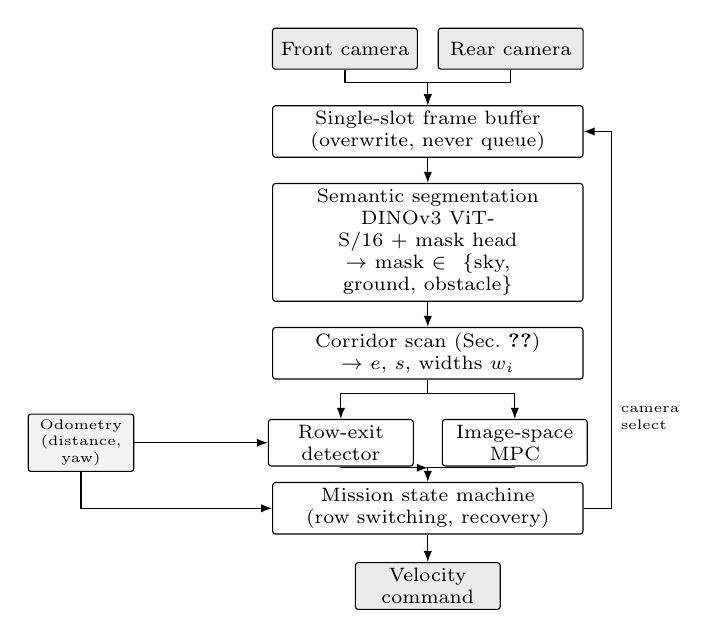
\begin{tikzpicture}[
  font=\scriptsize,
  node distance=3.2mm,
  box/.style={draw, rounded corners=1pt, align=center, inner sep=2pt,
              minimum height=5.2mm, text width=38mm},
  small/.style={box, text width=17mm},
  side/.style={box, text width=12mm, font=\tiny, fill=black!5},
  io/.style={box, text width=17mm, fill=black!8},
  ar/.style={-{Latex[length=1.4mm]}, thin}
]
\node[io] (camf) {Front camera};
\node[io, right=2.5mm of camf] (camr) {Rear camera};
\node[box, below=4.5mm of $(camf.south)!0.5!(camr.south)$] (buf)
      {Single-slot frame buffer\\(overwrite, never queue)};
\node[box, below=of buf] (seg)
      {Semantic segmentation\\DINOv3 ViT-S/16 + mask head\\$\rightarrow$ mask $\in\{$sky, ground, obstacle$\}$};
\node[box, below=of seg] (cen)
      {Corridor scan (Sec.~\ref{sec:centerline})\\$\rightarrow$ $e$, $s$, widths $w_i$};
\node[small, below left=5mm and -18mm of cen] (det) {Row-exit\\detector};
\node[small, below right=5mm and -18mm of cen] (mpc) {Image-space\\MPC};
\node[box, below=13mm of cen] (fsm) {Mission state machine\\(row switching, recovery)};
\node[io, below=3.5mm of fsm] (out) {Velocity command};
\node[side] (odo) at ([xshift=-33mm]det.center) {Odometry\\(distance, yaw)};
\draw[ar] (camf.south) -- ++(0,-1.6mm) -| (buf.north);
\draw[ar] (camr.south) -- ++(0,-1.6mm) -| (buf.north);
\draw[ar] (buf) -- (seg);
\draw[ar] (seg) -- (cen);
\draw[ar] (cen.south) -- ++(0,-1.8mm) -| (mpc.north);
\draw[ar] (cen.south) -- ++(0,-1.8mm) -| (det.north);
\draw[ar] (mpc.south) |- ($(fsm.north)+(0,1.8mm)$) -- (fsm.north);
\draw[ar] (det.south) |- ($(fsm.north)+(0,1.8mm)$);
\draw[ar] (odo.east) -- (det.west);
\draw[ar] (odo.south) |- (fsm.west);
\draw[ar] (fsm) -- (out);
\draw[ar] (fsm.east) -- ++(3.5mm,0) |- (buf.east)
      node[pos=0.12, right, font=\tiny, align=left] {camera\\select};
\end{tikzpicture}
\caption{AIAgNav processing pipeline. A single camera frame is segmented into
sky, traversable ground, and obstacle; a scan-row geometry stage reduces the
mask to a lateral error and a heading proxy, which drive the image-space MPC;
the same scan feeds the row-exit detector, and the mission state machine
sequences row following, headland turns, and blocked-row recovery.}
\label{fig:pipeline}
\end{figure}

%%=====================================================================
%% III. SYSTEM DESIGN
%%=====================================================================
\section{System Design}
\label{sec:design}

\begin{table}[t]
\caption{Summary of Notations}
\label{tab:notation}
\centering
\begin{tabular}{ll}
\toprule
Symbol & Description \\
\midrule
$H,\,W$ & Mask height and width, px \\
$c_x$ & Image centre column, $W/2$ \\
$f_i,\,\lambda_i$ & Height fraction and pooling weight of scan row $i$ \\
$x_{L,i},\,x_{R,i}$ & Corridor bounds on scan row $i$ \\
$x_{\mathrm{mid},i},\,w_i$ & Corridor midpoint and width on scan row $i$ \\
$e_i,\,e$ & Per-row and pooled normalized lateral error \\
$s$ & Heading proxy (slope term) \\
$\tau,\,\tau_{\min}$ & Traversable fraction of lower half; its threshold \\
$\mathbf{x},\,u$ & MPC state $[\,e\;\,s\,]^{\!\top}$ and control $u=\omega$ \\
$A,\,B$ & System and input matrices \\
$\alpha,\,\beta$ & Lateral coupling and control effectiveness \\
$Q,\,r,\,r_\Delta$ & State, control, and control-rate weights \\
$N,\,dt,\,dt_0$ & Horizon, control period, reference period \\
$\omega_{\max},\,\Delta\omega_{\max}$ & Angular rate and slew limits \\
$v$ & Commanded linear velocity \\
$m,\,\Delta_k$ & Exit evidence and its per-frame increment \\
$\rho,\,m_c$ & Evidence leak ratio and confirmation threshold \\
\bottomrule
\end{tabular}
\end{table}

\subsection{Semantic Segmentation}
The navigation state is derived from a per-pixel semantic segmentation of a
single forward-facing RGB frame. Under a corn canopy the appearance cues that
separate drivable ground from crop are unstable: illumination changes by more
than an order of magnitude between direct sun and deep shade within one row,
hanging leaves throw high-contrast shadows across the corridor floor, and soil
colour shifts with moisture and tillage. Hand-tuned colour or texture thresholds
are adequate over a short segment but do not survive these transitions, and the
row-following controller carries no independent state estimate to fall back on
when they fail. The system therefore learns the ground/crop distinction rather
than specifying it.

The network pairs a DINOv3~\cite{simeoni2025dinov3} ViT-S/16
backbone~\cite{ref14} with an encoder-only mask transformer head~\cite{ref16}.
The choice is driven by label efficiency rather than by accuracy on a public
benchmark. Annotated data for this task cannot be inherited from an existing
dataset: it must be produced by hand from footage recorded in the target field,
at the growth stage and camera mounting of the deployed robot, and the
achievable quantity is bounded by how much one operator can label in a season.
The training set here is 443 annotated frames, split $80/20$ between training
and validation, curated to cover the cases that break a row follower rather than
the average frame: entering a row, dead-end rows, gaps where plants are missing,
and downed corn. Self-supervised features of this family transfer to dense
prediction under very little supervision~\cite{ref15}, which is what makes a set
of that size viable; a backbone trained from scratch, or one supervised on
ImageNet classification, would demand substantially more annotation before
producing masks clean enough to measure corridor boundaries on. ViT-S/16 is the
smallest variant in the family, which matters because one set of weights must
serve both robots in the fleet, only one of which carries a GPU. Measured
segmentation quality on the held-out split is 0.8717 mIoU.

The model predicts three classes: sky, traversable ground, and obstacle. The
controller reads only the traversable class, so the presence of a sky class
deserves an explanation. At a row end, and throughout a headland, the upper part
of the frame opens onto bright sky. A two-class model must assign those pixels
to either ground or crop, and their brightness and near-absence of texture make
them resemble open ground far more closely than they resemble a corn plant.
Because the exit detector of Section~\ref{sec:exit} fires when the traversable
corridor widens toward the full image width, folding sky into the traversable
class reproduces the exact signature of a row end at arbitrary points inside a
row. A dedicated sky label removes that failure mode for the cost of one output
channel. The obstacle class, conversely, is deliberately coarse: it covers the
corn plants bounding the corridor, fallen stalks, and any foreign object,
because the control decision they induce is identical---do not drive there.
Separating them would add annotation burden without changing a single command.

At inference the model is given the full-resolution camera frame and returns a
class-index mask, which is resized to the frame resolution when the two differ.
That resize must be nearest-neighbour. Mask values are class indices, not
intensities, so any interpolating kernel synthesises intermediate values that
correspond to no class at all, and it does so precisely at region
boundaries---which is exactly where Section~\ref{sec:centerline} measures the
corridor edges. A single misplaced boundary column biases the lateral error for
that frame.

\subsection{Corridor and Centerline Estimation}
\label{sec:centerline}
The mask is reduced to a two-dimensional navigation state by pure geometry. No
regression head is trained to predict heading or lateral distance, and no camera
intrinsics enter the computation: the state is read directly off the class mask,
so it is defined in normalized image coordinates and is independent of camera
resolution.

The system measures the corridor on a small set of horizontal scan rows
(Fig.~\ref{fig:overlay}) placed at fractions $f_i$ of the image height, ordered
from farthest to nearest. On each scan row it starts at the image centre column
$c_x$ and expands outward while the mask remains traversable, giving the bounds
$x_{L,i}$ and $x_{R,i}$ of the contiguous traversable run that straddles the
centre column. Each valid scan row then gives a lateral error, normalized by the
half-width so that it is dimensionless and bounded, and these are pooled into a
single lateral state $e$ by a weighted mean over the valid rows,
\begin{align}
x_{\mathrm{mid},i} &= \tfrac{1}{2}\left(x_{L,i}+x_{R,i}\right),
   \qquad w_i = x_{R,i}-x_{L,i}, \nonumber\\
e_i &= \frac{x_{\mathrm{mid},i}-c_x}{W/2}, \nonumber\\
e   &= \mathrm{clip}\!\left(
       \frac{\sum_i \lambda_i e_i}{\sum_i \lambda_i},\; -1,\; 1 \right),
       \nonumber\\
s   &= e_{\mathrm{far}} - e_{\mathrm{near}}.
\label{eq:state}
\end{align}
Anchoring the search at $c_x$ rather than taking the widest traversable run in
the row is what makes the measurement unambiguous when the mask contains more
than one open region, as it does whenever a gap in the crop wall exposes the
neighbouring row: the corridor the robot is actually in is the one aligned with
its own heading. If the centre column is not traversable, that scan row yields
no measurement and is skipped. The width $w_i$ is retained and consumed by the
exit detector of Section~\ref{sec:exit}.

A positive $e$ places the corridor midpoint right of the image centre, meaning
the robot sits left of the corridor centre. The weights $\lambda_i$ favour the
near rows, because near and far rows fail in opposite ways: the near rows report
where the robot is now and segment cleanly, whereas the far rows carry the
earliest warning of a curve or a row end but sit where perspective compresses
the corridor to a few pixels. Weighting toward the near field keeps steering
stable while leaving the far rows enough influence to anticipate.

Because the same scan already yields an offset at several distances, the robot's
heading relative to the row follows from their difference at no additional cost.
The slope term $s$ is evaluated between the farthest and nearest valid rows: a
corridor that tilts rightward with distance indicates the robot is heading left
of the row direction. This is the term that separates the two ways a robot can
be wrong inside a row---displaced from the centreline, and pointed across
it---which a single lateral reading cannot distinguish. It is computed across
rows within one frame rather than across time, so it needs no history, no filter
and no inertial measurement. Under a pinhole model the pair $(e,s)$ is an
invertible linear transform of the physical (lateral offset, heading error)
pair, so no navigation information is lost by never leaving image space.

A frame is accepted only if at least one scan row produced a measurement and the
traversable fraction $\tau$ of the lower half of the mask reaches a threshold
$\tau_{\min}$. The second test rejects the case where the mask has
collapsed---an occluded lens, a lost row---while a narrow spurious run at the
centre column still yields a confident-looking midpoint. On rejection the
controller holds its previous command rather than steering on the frame, and
stops if rejections persist.

%%---------------------------------------------------------------------
%% Fig. 2 -- segmentation overlay.  PLACEHOLDER.
%% To use a real image: drop the file into the Overleaf project, then
%% replace the \framebox line below with
%%     \includegraphics[width=\columnwidth]{overlay.png}
%%---------------------------------------------------------------------
\begin{figure}[t]
\centering
\framebox[0.98\columnwidth]{\rule{0pt}{3.6cm}\parbox{0.7\columnwidth}{\centering
\textbf{[Fig.~2 placeholder]}\\[2pt] segmentation overlay:\\ scan rows, corridor
bounds, midpoints}}
\caption{Corridor measurement on a class mask. The traversable region is washed
over the camera frame; on each scan row the search starts at the image centre
column and expands outward to the corridor bounds, whose midpoint gives the
per-row lateral error. The difference between the far and near rows is the
heading proxy.}
\label{fig:overlay}
\end{figure}

\subsection{Model Predictive Row Following}
\label{sec:mpc}
The controller converts the state $(e,s)$ into an angular velocity. A
proportional law on $e$ alone is sufficient to hold a straight row but couples
poorly to the heading term, and it offers no principled way to bound how sharply
the command may change between frames---a real constraint here, since a single
badly segmented frame must not produce a step in steering. The system therefore
uses a receding-horizon model predictive controller~\cite{ref17}, which
expresses both requirements as costs and constraints on the same optimization.

The state is $\mathbf{x} = [\,e\;\,s\,]^{\!\top}$ and the control is the angular
velocity $u=\omega$. The cost penalizes deviation from the row over the horizon
$N$ while regularizing the command,
\begin{equation}
J = \sum_{k=1}^{N} \mathbf{x}_k^{\!\top} Q\, \mathbf{x}_k
  + \sum_{k=0}^{N-1} \left[ r\,u_k^2
  + r_\Delta \left(u_k-u_{k-1}\right)^2 \right],
\label{eq:cost}
\end{equation}
with $Q=\mathrm{diag}(q_e,q_s)$. The two state weights encode a priority: being
off-centre is penalized considerably more than being misaligned, because a
heading error corrects itself as the robot advances whereas a lateral offset
does not. The term in $r$ discourages large commands, and the term in $r_\Delta$
penalizes change between consecutive commands. That last term is what supplies
temporal smoothing in this system. Learned under-canopy controllers typically
obtain smoothing by fusing the visual estimate with inertial measurements in a
Kalman filter~\cite{sivakumar2021cropfollow}; here it falls out of the cost
function, so the pipeline needs neither an IMU nor a filter state that must be
re-initialized whenever the mission is paused.

Over one control period the corridor midpoint drifts laterally in proportion to
the current heading error, and the heading error itself is driven by the
commanded rate. The state is updated by a linear time-invariant model in
normalized image space, subject to a magnitude bound and a slew bound on the
command,
\begin{align}
\mathbf{x}_{k+1} &= A\,\mathbf{x}_k + B\,u_k, \nonumber\\
A &= \begin{bmatrix} 1 & \alpha \\ 0 & 1 \end{bmatrix},
\qquad
B = \begin{bmatrix} 0 \\ \beta \end{bmatrix}, \nonumber\\
\left|u_k\right| &\le \omega_{\max},
\qquad
\left|u_k-u_{k-1}\right| \le \Delta\omega_{\max}.
\label{eq:mpc}
\end{align}
Here $\alpha$ is the lateral coupling---how much heading error translates into
lateral drift per step---and $\beta$ is the control effectiveness, how much the
commanded rate moves the heading term per step. Both are identified empirically.
This is a point of departure from range-view systems such as
P-AgNav~\cite{kim2025pagnav}, where a $360^{\circ}$ horizontal field of view
maps angular velocity to image displacement in closed form. A perspective camera
admits no such constant: the pixel displacement produced by a given rotation
depends on depth, which is unobserved. Fitting the two scalars on logged runs
avoids requiring the depth that would make them analytic. In~\eqref{eq:mpc},
$u_{-1}$ is the command applied on the previous frame, so the slew constraint
binds across frames and not merely within the planned sequence. The problem is
solved by sequential least-squares quadratic programming at every accepted
frame; only the first element $u_0$ is applied, and the remainder of the horizon
is discarded and recomputed on the next frame.

One practical requirement shapes the parameterization. The same controller runs
on two robots whose inference rates differ by more than an order of magnitude,
and a model calibrated per \emph{step} is wrong on both unless the step is
fixed. The parameters $\alpha$, $\beta$ and $\Delta\omega_{\max}$ are therefore
specified at a reference control period $dt_0$ and scaled by $dt/dt_0$ at
construction. The per-step drift and control effectiveness then match the real
elapsed time per step, and the slew limit stays constant in
$\mathrm{rad}\,\mathrm{s}^{-2}$ rather than silently tightening as the loop
slows.

The linear velocity is held at a constant cruise value while the robot is
following a row. This is a deliberate simplification relative to
P-AgNav~\cite{kim2025pagnav}, which couples speed inversely to commanded
curvature so the platform slows through sharp corrections. Under the row
geometry considered here the commanded rate stays small enough that the coupling
changes little, and a constant speed makes the distance-based logic of
Section~\ref{sec:exit} easier to reason about. Speed is reduced only during the
headland manoeuvre, where overshoot is most costly.

\subsection{Row Exit Detection}
\label{sec:exit}
The system recognizes two end-of-row signatures, both read from quantities
Section~\ref{sec:centerline} has already computed. In the open signature the
corridor widens from the narrow band characteristic of an occupied row toward
the full image width, and the outer strips at the image borders become
traversable: the crop walls have ended. The test requires a sufficient number of
scan rows to be simultaneously wide and flank-clear, but deliberately does not
require \emph{particular} rows. Requiring the far rows is the intuitive choice
and fails in the field, because beyond the last plants the distant ground
segments poorly and those rows can remain invalid indefinitely. In the blocked
signature no scan row yields a corridor at all while the lower half of the mask
still contains obstacle pixels, which is a crop wall square ahead rather than a
lost mask.

Neither signature may be trusted on a single frame, and the debounce is where
the design matters. Evidence accumulates in \emph{physical} units rather than in
frames,
\begin{equation}
m_{k+1} =
\begin{cases}
  m_k + \Delta_k, & \text{signature present},\\[2pt]
  \max\!\left(m_k - \rho\,\Delta_k,\; 0\right), & \text{otherwise},
\end{cases}
\label{eq:accumulator}
\end{equation}
firing when $m_k \ge m_c$. The increment $\Delta_k$ is the distance driven since
the previous frame for the open signature and the elapsed time for the blocked
signature. The units differ because the two signatures fail differently: an exit
must be confirmed by driving through it, so if the robot stalls the safe outcome
is not to fire, whereas a blocked view stops the robot outright, so a
distance-based counter would never fill and the recovery would deadlock.

Counting frames instead would not be a simplification but a defect: the same
count means more than a second of evidence on the CPU-only robot and a fraction
of one on the GPU robot, so a mid-row gap that is harmless on one fires an exit
on the other. Nor may the accumulator demand strictly consecutive frames, since
a single flickering frame would then reset a streak spanning tens of them. The
leak is asymmetric, $\rho<1$, because a symmetric leak sounds neutral and is
not: a signature holding on half the frames nets exactly zero and can never fire
however far the robot drives, which is precisely what a real but marginal exit
looks like.

Each signature is armed by distance travelled into the row---the open signature
only after the robot is far enough in that the open field behind it has left the
frame, the blocked signature much earlier, since an obstacle just past the row
entrance must still be caught and that signature cannot false-fire there. When
an exit fires, the row-entry distance is back-dated to the start of the evidence
streak rather than to the confirming frame, so the confirmation distance is not
charged twice against the headland manoeuvre that follows.

\subsection{Row Switching}
\label{sec:switching}
Multi-row operation is sequenced by a finite state machine,
Fig.~\ref{fig:fsm}. On a confirmed open exit the robot leaves row following and
drives clear of the last plants, then executes a quarter turn onto the headland,
traverses to the neighbouring row, turns again to face down it, and reacquires
row following once the segmentation mask presents a corridor. The two turns and
the traverse are closed on wheel odometry rather than on vision, because the
headland offers no corridor to steer by; each turn terminates on accumulated
swept yaw rather than on elapsed time, and vision resumes as the authority the
moment the robot is inside the next row. Turn direction alternates between
switches, so the robot covers the plot in a boustrophedon pattern, and the
mission ends after a commanded number of rows or when reacquisition finds no
corridor, which is how an unbounded mission recognizes that no rows are left.

The clearing leg runs slower than the row-following cruise, since overshoot
there is what misaligns the entry into the next row. Where a rear camera is
available, that leg is steered from the rear view looking back down the row just
left, which reports directly whether the tail has cleared the last plants; the
conversion from the rear view to the same state used in Section~\ref{sec:mpc} is
not a sign flip. A false exit is made cheap rather than made impossible: if the
robot has left row following but the nearest scan row still reports crop on both
flanks over a short distance, the exit is revoked and row following resumes with
the row count unchanged.

The blocked signature enters a separate branch. Because the system drives only
forward within a row, a crop wall ahead cannot be turned around in place without
striking plants, so the robot reverses out of the end it entered under rear-view
guidance and odometry bounds, then joins the next row with an S-turn. That row
is traversed in the same direction as the blocked one rather than the
alternating direction, since the robot never reached the far end, and the
boustrophedon flip is suppressed once to account for it. Blocked events are
counted and reported at mission completion, as they mark rows that were not
fully covered. The branch is gated on the presence of the rear camera; without
it a blocked signature stops the robot and ends the mission.

%%---------------------------------------------------------------------
%% Fig. 3 -- mission state machine (TikZ, drawn inline).
%% Uses figure* so it spans both columns -- it is 75mm wide.
%%---------------------------------------------------------------------
\begin{figure}[t]
\centering
\resizebox{\columnwidth}{!}{%
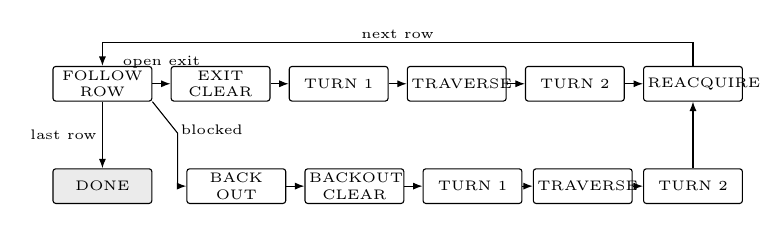
\begin{tikzpicture}[
  font=\tiny,
  st/.style={draw, rounded corners=1pt, align=center, inner sep=1.5pt,
             minimum height=4.4mm, text width=11.5mm},
  term/.style={st, fill=black!8},
  ar/.style={-{Latex[length=1.2mm]}, thin},
  lbl/.style={font=\tiny, inner sep=1pt}
]
\node[st] (f)  at (0,0)    {FOLLOW\\ROW};
\node[st] (ec) at (15mm,0) {EXIT\\CLEAR};
\node[st] (t1) at (30mm,0) {TURN 1};
\node[st] (tr) at (45mm,0) {TRAVERSE};
\node[st] (t2) at (60mm,0) {TURN 2};
\node[st] (ra) at (75mm,0) {REACQUIRE};
\node[term] (dn) at (0,-13mm)    {DONE};
\node[st]  (bo)  at (17mm,-13mm) {BACK\\OUT};
\node[st]  (bc)  at (32mm,-13mm) {BACKOUT\\CLEAR};
\node[st]  (b1)  at (47mm,-13mm) {TURN 1};
\node[st]  (btr) at (61mm,-13mm) {TRAVERSE};
\node[st]  (b2)  at (75mm,-13mm) {TURN 2};
\draw[ar] (f)  -- node[lbl, above=1.6mm] {open exit} (ec);
\draw[ar] (ec) -- (t1);
\draw[ar] (t1) -- (tr);
\draw[ar] (tr) -- (t2);
\draw[ar] (t2) -- (ra);
\draw[ar] (ra.north) -- ++(0,3mm) -- node[lbl, above] {next row} ($(f.north)+(0,3mm)$) -- (f.north);
\draw[ar] (f.south) -- node[lbl, left=0.3mm] {last row} (dn.north);
\draw[ar] (f.south east) -- node[lbl, pos=0.9, right=0.3mm] {blocked} ++(3.2mm,-4mm) |- (bo.west);
\draw[ar] (bo)  -- (bc);
\draw[ar] (bc)  -- (b1);
\draw[ar] (b1)  -- (btr);
\draw[ar] (btr) -- (b2);
\draw[ar] (b2.north) -- (ra.south);
\end{tikzpicture}}
\caption{Mission state machine. The upper chain is the nominal cycle: a
confirmed open exit sends the robot across the headland and back into row
following. The lower chain is the blocked-row branch, which reverses out of the
row and joins the next one in the same direction of travel. The mission
terminates after the commanded number of rows, and also when reacquisition finds
no corridor, which is how an unbounded mission recognizes that no rows are
left.}
\label{fig:fsm}
\end{figure}

%%=====================================================================
%% IV. EXPERIMENTAL RESULTS  -- RESERVED, deferred until field data exists.
%% Tables II-IV are laid out so the page budget is honest. Fill the
%% dashes; do not fabricate.
%%=====================================================================
\section{Experimental Results}
\label{sec:results}
Experiments are conducted to demonstrate the capabilities of the proposed system
across cornfield scenarios in both simulation and a real cornfield, referred to
as SIM and ACRE (the Agronomy Center for Research and Education at Purdue)
respectively, matching the evaluation structure of~\cite{kim2025pagnav}.

Performance is evaluated on three criteria. The first two
follow~\cite{kim2025pagnav}: collisions with crops, counted under the same
definition, and human interventions. The third is meters between interventions
(MDBI), defined as the distance driven autonomously divided by the number of
interventions, where an intervention is a joystick takeover by the supervising
operator and takeover distance is subtracted rather than credited to the
controller. MDBI is reported because it is the figure the field literature
compares on, and because unlike a normalized image-space tracking error it is
expressed in metres and is independent of camera mounting. A run with zero
interventions yields only a lower bound on MDBI, so trials are pooled---distances
summed, interventions summed---before a figure is quoted.

\TODO{Write this section from field data. Fill Tables II--IV, state the
perception result (0.8717 mIoU on the held-out split of 443 frames), and add the
field-challenge figure matching Fig.~7 of~\cite{kim2025pagnav}. Do not report
the simulation runs as field results: they have zero interventions, so MDBI from
them is a lower bound with no denominator.}

\begin{table}[t]
\caption{Specifications of Experimental Environments}
\label{tab:envs}
\centering
\begin{tabular}{lcc}
\toprule
 & SIM & ACRE \\
\midrule
Row spacing (m)        & --- & --- \\
Row length (m)         & --- & --- \\
Growth stage           & --- & --- \\
Camera mount           & --- & --- \\
Compute variant        & --- & --- \\
Cruise speed (m/s)     & --- & --- \\
$\omega_{\max}$ (rad/s) & --- & --- \\
\bottomrule
\end{tabular}
\end{table}

\begin{table}[t]
\caption{Navigation Performance in SIM}
\label{tab:sim}
\centering
\begin{tabular}{lccccc}
\toprule
Trial & Rows & Completed & Collisions & Interv. & Blocked \\
\midrule
--- & --- & --- & --- & --- & --- \\
--- & --- & --- & --- & --- & --- \\
\midrule
Total & --- & --- & --- & --- & --- \\
\bottomrule
\end{tabular}
\end{table}

\begin{table}[t]
\caption{Navigation Performance in ACRE}
\label{tab:acre}
\centering
\begin{tabular}{lccccc}
\toprule
Trial & Rows & Dist. (m) & Collisions & Interv. & MDBI (m) \\
\midrule
--- & --- & --- & --- & --- & --- \\
--- & --- & --- & --- & --- & --- \\
\midrule
Pooled & --- & --- & --- & --- & --- \\
\bottomrule
\end{tabular}
\end{table}

%%=====================================================================
%% V. CONCLUSION
%%=====================================================================
\section{Conclusion}
This paper presented AIAgNav, a navigation system that drives a ground robot
in-row and under-canopy in cornfields, and across multiple rows, from a single
monocular RGB camera. The navigation state is recovered from a semantic
segmentation mask by closed-form geometry and consumed directly by a model
predictive controller formulated in normalized image coordinates, so the
pipeline uses no GNSS, no map, no waypoints, no LiDAR, no camera calibration and
no state estimator between perception and control. A mission layer detects the
end of a row from the same mask, sequences headland turns, and recovers from
blocked rows by reversing out under rear-view guidance. Expressing end-of-row
evidence in metres and seconds rather than in frame counts allows one set of
thresholds to transfer between robots whose inference rates differ by an order
of magnitude, which is what makes the same system deployable on a GPU-equipped
platform and on a stock CPU-only one.

Three directions follow. The first is above-canopy transit: an RTK receiver used
only between the field edge and the row entrance, the one regime in which GNSS
is dependable, would close the gap between deployment and the first row. The
second is integration with the physical sampling module the platform already
carries, so that a covered plot yields measurements rather than a trajectory.
The third is the sky class, which the controller currently ignores: a lens
occluded by a leaf and a crop wall directly ahead produce the same mask today,
and sky visibility is the most direct signal available for separating them.

%%=====================================================================
%% REFERENCES
%%
%% Written as a thebibliography environment on purpose: no .bib file and
%% no BibTeX pass, so this cannot fail on Overleaf.
%%
%% [1]-[6] are verified. ref07-ref18 are RESERVED SLOTS holding the page
%% space a real list needs -- replace each with the actual citation.
%% Do not hand-write bibliographic data; pull it from the source.
%%=====================================================================
\begin{thebibliography}{99}

\bibitem{kim2025pagnav}
K.~Kim, A.~Deb, and D.~J. Cappelleri, ``P-AgNav: Range view-based autonomous
navigation system for cornfields,'' \emph{IEEE Robot. Autom. Lett.}, vol.~10,
no.~4, pp. 3366--3373, Apr. 2025.

\bibitem{kim2022pagbot}
K.~Kim, A.~Deb, and D.~J. Cappelleri, ``P-AgBot: In-row \& under-canopy
agricultural robot for monitoring and physical sampling,'' \emph{IEEE Robot.
Autom. Lett.}, vol.~7, no.~3, pp. 7942--7949, Jul. 2022.

\bibitem{kim2024pagslam}
K.~Kim, A.~Deb, and D.~J. Cappelleri, ``P-AgSLAM: In-row and under-canopy SLAM
for agricultural monitoring in cornfields,'' \emph{IEEE Robot. Autom. Lett.},
vol.~9, no.~6, pp. 4982--4989, Jun. 2024.

\bibitem{panda2023agronav}
S.~K. Panda, Y.~Lee, and M.~K. Jawed, ``Agronav: Autonomous navigation framework
for agricultural robots and vehicles using semantic segmentation and semantic
line detection,'' in \emph{Proc. IEEE/CVF Conf. Comput. Vis. Pattern Recognit.
Workshops}, 2023, pp. 6272--6281.

\bibitem{sivakumar2021cropfollow}
A.~N. Sivakumar, S.~Modi, M.~V. Gasparino, C.~Ellis, A.~E. Baquero Velasquez,
G.~Chowdhary, and S.~Gupta, ``Learned visual navigation for under-canopy
agricultural robots,'' in \emph{Proc. Robotics: Science and Systems}, 2021.

\bibitem{simeoni2025dinov3}
O.~Sim\'{e}oni, H.~V. Vo, M.~Seitzer, F.~Baldassarre, M.~Oquab, C.~Jose,
V.~Khalidov, M.~Szafraniec, S.~Yi, M.~Ramamonjisoa, \emph{et al.}, ``DINOv3,''
\emph{arXiv:2508.10104}, 2025.

\bibitem{ref07}
\TODO{precision agriculture / remote sensing review}

\bibitem{ref08}
\TODO{Internet of Things for precision agriculture (IoT4Ag)}

\bibitem{ref09}
\TODO{agricultural robotics survey; aerial vs. ground platform trade-off}

\bibitem{ref10}
\TODO{GNSS-based agricultural navigation}

\bibitem{ref11}
\TODO{GNSS-based agricultural navigation, second entry}

\bibitem{ref12}
\TODO{review of classical path-planning strategies for mobile robots}

\bibitem{ref13}
\TODO{crop-row detection from images in maize fields}

\bibitem{ref14}
\TODO{vision transformers for image recognition at scale}

\bibitem{ref15}
\TODO{self-supervised dense visual representation learning (DINOv2)}

\bibitem{ref16}
\TODO{encoder-only mask transformer segmentation head (EoMT)}

\bibitem{ref17}
\TODO{model predictive control for mobile robot trajectory tracking}

\bibitem{ref18}
\TODO{under-canopy phenotyping / crop monitoring platform}

\end{thebibliography}

\end{document}
